\documentclass[]{article}
\usepackage{tikz}
\usepackage{amsmath}
\usepackage{minted}

%opening
\title{Candlestick encoding}
\author{Reindeer Flotilla}

\begin{document}

\maketitle
\tableofcontents

\section{Nomenclature}

The principal components that we consider in a candlestick diagram are the candles. They look like the drawing below, where its main parts are named body and shadows.

\begin{center}
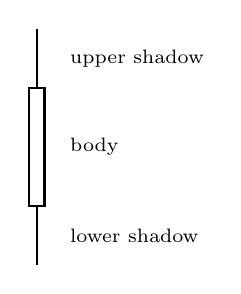
\begin{tikzpicture}
\filldraw[thick, fill=white] (0, 0.75)rectangle node[right] {\scriptsize \hspace{2mm} body} (0.2, 2.25) ;
\draw[thick] (0.1, 2.25) -- node[right] {\scriptsize \hspace{2mm} upper shadow} (0.1, 3) ;
\draw[thick] (0.1, 0.75) -- node[right] {\scriptsize \hspace{2mm} lower shadow}  (0.1, 0) ;
\end{tikzpicture}
\end{center}

Candlesticks are usually composed of the body (black / white or green / red), and an upper / lower shadows. The area between open and close is called the real \textbf{body}, price excursions above and below the real body are \textbf{shadows}. Shadows illustrate highest and lowest traded prices of a security during the time interval represented. Body illustrates the opening and closing trades.

The range between \textit{open} and \textit{close} the \textit{OC} range.

The particular range between any \textit{min} and \textit{max} in an individual tick will be called $\overline{mm}$.

To encode an OHLC tick and its corresponding candlestick, the following pieces of information are needed:

\begin{itemize}
	\item $\overline{MM}$ range between the absolute minimum and maximum values found in the entire time series. If \textit{min} $>$ \textit{max}, the body size will be negative.
	\item $\overline{mm}$ range between min and max values of any particular tick.
	\item Direction and length of change wrt. previous candlestick.
	\item Body position
	\item Upper shadow size.
	\item Lower shadow size.
\end{itemize}

All these elements result in a three-components encoding: $\overline{mm}$, body position and direction. The first three are encoded considering the previous element in the series. The result is 3-tuple that will encode candlestick dynamics. Size is relative to the previous elements, thus giving information about whether this candlestick is greater or smaller than previous one. Position is telling us how many shadows it has, whether the body is centered or shifted, and its relative size compared with the $\overline{mm}$ range. Finally, direction informs about whether this candlestick represents an increase or decrease of the different ranges with respect to the previous one.

\[
	\underbrace{SS}_\text{size} + \underbrace{BB}_\text{position} + \underbrace{DD}_\text{direction}
\]

\subsection{Normalization}

We must consider what is the maximum range found in the time series, between the \textit{min} and \textit{max} of an individual tick. Considering that range, we will normalized the entire time series. We will call the range between \textit{min} and \textit{max} the $\overline{MM}$ range. 

\section{High-Low range --Size}
\subsection{Absolute or relative Encoding}

To encode $\overline{mm}$ range size, it is possible to use \textbf{absolute} or \textbf{relative} encoding.
\begin{description}
	\item[Absolute] determines what the current range size with respect to the maximum range found in the series ($\overline{MM}$) as a discrete value for the percentage of $\overline{MM}$: 0, 10, 25, 50, 75, 100 or more.
	\item[Relative] encodes the body size as a percentage of the $\overline{mm}$ range, again, as a discrete value for the percentage of $\overline{mm}$: 0, 10, 25, 50, 75, 100 or more.
\end{description}

Relative encoding may refer to the percentage of change in size of the current candlestick with respect to the previous one. That way, encoding provides contextualized information about the current \textit{tick}, instead of simply informing about the individual characteristics of the element.

\subsection{Size encoding}

Options for the size encoding are:

\begin{minted}[numbersep=5pt,gobble=2,frame=lines,framesep=2mm]{bash}
  {P|N}{0..6}
\end{minted}

The first character indicates greater or smaller $\overline{mm}$ range with respect to the previous one, and the range between 0 and 6 indicates whether that increase/decrease of size is 0\%, 10\%, 25\%, 50\%, 75\%, 100\% or more.

\section{Candlestick body position}

\subsection{$\overline{OC} \neq$  0}

\subsubsection{Two-shadowed}

Let's start by those covering different ranges of the \textit{min}-\textit{max} range (10\%, 25\%, 50\%, 75\% and 100\%), and \textit{open}-\textit{close} range centered between them. By \textit{centered} we can assume that it can be considered as with equal-length shadows at both sides of the body.

\begin{center}
	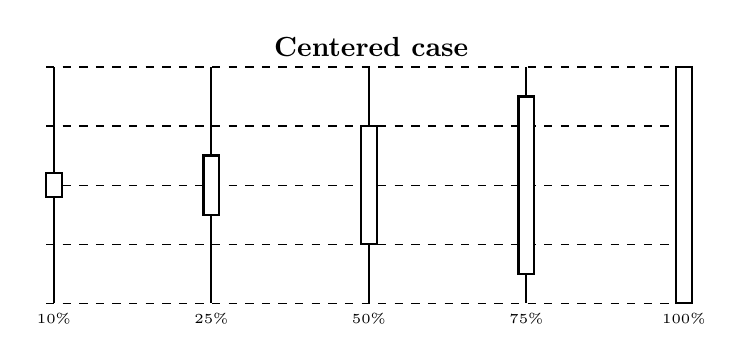
\begin{tikzpicture}
	\draw[dashed] (0,3) -- (8, 3);
	\draw[dashed] (0,2.25) -- (8, 2.25);
	\draw[dashed] (0,1.5) -- (8, 1.5);
	\draw[dashed] (0,0.75) -- (8, 0.75);
	\draw[dashed] (0,0) -- (8, 0);
	
	\filldraw[thick, fill=white] (0, 1.35)rectangle (0.2, 1.65);
	\draw[thick] (0.1, 1.65) -- (0.1, 3);
	\draw[thick] (0.1, 1.35) -- (0.1, 0) node[align=center, below] {\tiny 10\%};
	
	\filldraw[thick, fill=white] (2, 1.125)rectangle (2.2, 1.875);
	\draw[thick] (2.1, 1.875) -- (2.1, 3);
	\draw[thick] (2.1, 1.125) -- (2.1, 0) node[align=center, below] {\tiny 25\%};
	
	\filldraw[thick, fill=white] (4, 0.75)rectangle (4.2, 2.25);
	\draw[thick] (4.1, 2.25) -- (4.1, 3);
	\draw[thick] (4.1, 0.75) -- (4.1, 0) node[align=center, below] {\tiny 50\%};
	
	\filldraw[thick, fill=white] (6, 0.375)rectangle (6.2, 2.625);
	\draw[thick] (6.1, 2.625) -- (6.1, 3);
	\draw[thick] (6.1, 0.375) -- (6.1, 0) node[align=center, below] {\tiny 75\%};
	
	\filldraw[thick, fill=white] (8, 0)rectangle (8.2, 3);
	\draw[thick] (8.1, 0) -- (8.1, 0) node[align=center, below] {\tiny 100\%};
	\node[above, font=\bfseries] at (current bounding box.north) {Centered case};
\end{tikzpicture}
\end{center}

Now let's consider those candlesticks that are not centered but shifted either upwards/downwards. Base assumption is that the range \textit{open}-\textit{close} is 50\% of the range between \textit{min}-\textit{max}.

\begin{center}
	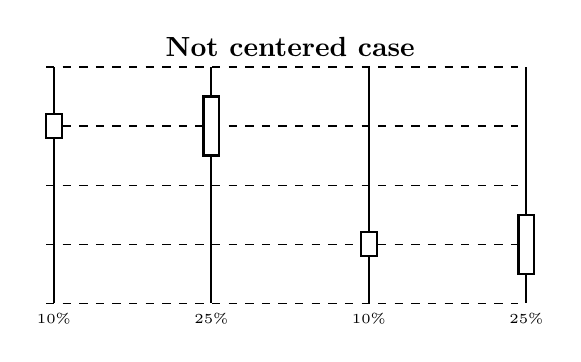
\begin{tikzpicture}
	\draw[dashed] (0,3) -- (6, 3);
	\draw[dashed] (0,2.25) -- (6, 2.25);
	\draw[dashed] (0,1.5) -- (6, 1.5);
	\draw[dashed] (0,0.75) -- (6, 0.75);
	\draw[dashed] (0,0) -- (6, 0);
	
	\filldraw[thick, fill=white] (0, 2.1)rectangle (0.2, 2.4);
	\draw[thick] (0.1, 2.4) -- (0.1, 3);
	\draw[thick] (0.1, 2.1) -- (0.1, 0) node[align=center, below] {\tiny 10\%};
	
	\filldraw[thick, fill=white] (2, 1.875)rectangle (2.2, 2.625);
	\draw[thick] (2.1, 2.625) -- (2.1, 3);
	\draw[thick] (2.1, 1.875) -- (2.1, 0) node[align=center, below] {\tiny 25\%};
	
	\filldraw[thick, fill=white] (4, 0.6)rectangle (4.2, 0.9);
	\draw[thick] (4.1, 0.9) -- (4.1, 3);
	\draw[thick] (4.1, 0.6) -- (4.1, 0) node[align=center, below] {\tiny 10\%};
	
	\filldraw[thick, fill=white] (6, 0.375)rectangle (6.2, 1.125);
	\draw[thick] (6.1, 1.125) -- (6.1, 3);
	\draw[thick] (6.1, 0.375) -- (6.1, 0) node[align=center, below] {\tiny 25\%};
	\node[above, font=\bfseries] at (current bounding box.north) {Not centered case};
	\end{tikzpicture}
\end{center}

\subsubsection{One-shadow}

Now, consider ranges between \textit{open}-\textit{close} that exceed the 50\% limit, so they are on values around 75\% of the \textit{min}-\textit{max} range.

\begin{center}
	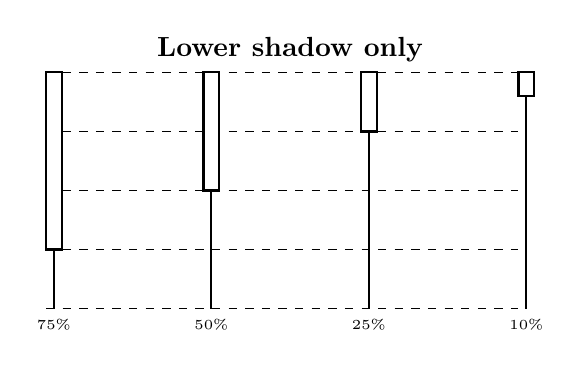
\begin{tikzpicture}
	\draw[dashed] (0,3) --      (6, 3);
	\draw[dashed] (0,2.25) -- (6, 2.25);
	\draw[dashed] (0,1.5) --   (6, 1.5);
	\draw[dashed] (0,0.75) -- (6, 0.75);
	\draw[dashed] (0,0) --      (6, 0);
	
	\filldraw[thick, fill=white] (0, 0.75)rectangle (0.2, 3);
	\draw[thick] (0.1, 3) -- (0.1, 3);
	\draw[thick] (0.1, 0.75) -- (0.1, 0) node[align=center, below] {\tiny 75\%};
	
	\filldraw[thick, fill=white] (2, 1.5)rectangle (2.2, 3);
	\draw[thick] (2.1, 3)   -- (2.1, 3);
	\draw[thick] (2.1, 1.5) -- (2.1, 0) node[align=center, below] {\tiny 50\%};
	
	\filldraw[thick, fill=white] (4, 2.25)rectangle (4.2, 3);
	\draw[thick] (4.1, 3) -- (4.1, 3);
	\draw[thick] (4.1, 2.25) -- (4.1, 0) node[align=center, below] {\tiny 25\%};
	
	\filldraw[thick, fill=white] (6, 2.7)rectangle (6.2, 3);
	\draw[thick] (6.1, 3) -- (6.1, 3);
	\draw[thick] (6.1, 2.7) -- (6.1, 0) node[align=center, below] {\tiny 10\%};
	\node[above, font=\bfseries] at (current bounding box.north) {Lower shadow only};
	\end{tikzpicture}
\end{center}

\begin{center}
	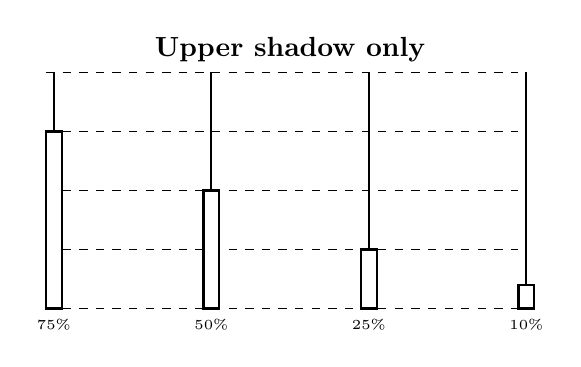
\begin{tikzpicture}
	\draw[dashed] (0,3) --      (6, 3);
	\draw[dashed] (0,2.25) -- (6, 2.25);
	\draw[dashed] (0,1.5) --   (6, 1.5);
	\draw[dashed] (0,0.75) -- (6, 0.75);
	\draw[dashed] (0,0) --      (6, 0);
	
	\filldraw[thick, fill=white] (0, 0)rectangle (0.2, 2.25);
	\draw[thick] (0.1, 2.25) -- (0.1, 3);
	\draw[thick] (0.1, 0) -- (0.1, 0) node[align=center, below] {\tiny 75\%};
	
	\filldraw[thick, fill=white] (2, 0)rectangle (2.2, 1.5);
	\draw[thick] (2.1, 1.5) -- (2.1, 3);
	\draw[thick] (2.1, 0) -- (2.1, 0) node[align=center, below] {\tiny 50\%};
	
	\filldraw[thick, fill=white] (4, 0)rectangle (4.2, 0.75);
	\draw[thick] (4.1, 0.75) -- (4.1, 3);
	\draw[thick] (4.1, 0) -- (4.1, 0) node[align=center, below] {\tiny 25\%};

	\filldraw[thick, fill=white] (6, 0)rectangle (6.2, 0.3);
	\draw[thick] (6.1, 0.3) -- (6.1, 3);
	\draw[thick] (6.1, 0) -- (6.1, 0) node[align=center, below] {\tiny 10\%};
	\node[above, font=\bfseries] at (current bounding box.north) {Upper shadow only};
	\end{tikzpicture}
\end{center}

\subsubsection{Zero-shadows}

It is also possible that $\overline{mm}$ ranges matches the \textit{OC} range. In that case we find zero shadows or complete match between the open-close interval and the min-max.

In that case, body position and size might be encoded with respect to the maximum $\overline{mm}$ range, but that will not add information about the current position in the trade. Alternatively, \textit{ticks} with zero shadows will be encoded only by the body size. Shadows and position will be considered as zero.

\subsection{$\overline{OC}$ = 0}

The case where $\overline{mm}$ is zero corresponds to an almost non-existent body. To correctly compute this case, it is proposed to consider null body when its \textit{OC} range is less than 1-2\% of the $\overline{mm}$ range.

\begin{center}
	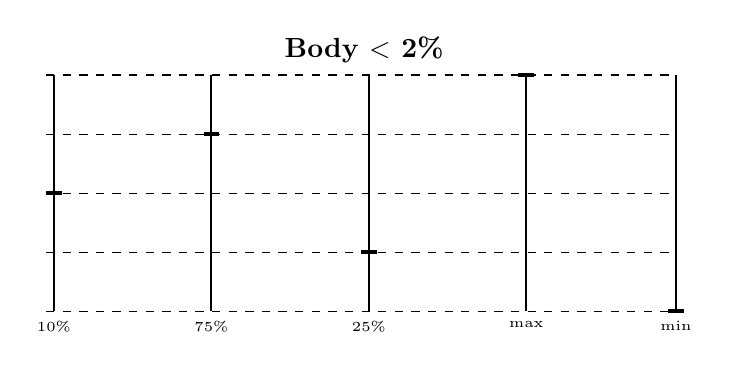
\begin{tikzpicture}
	\draw[dashed] (0,3) -- (8, 3);
	\draw[dashed] (0,2.25) -- (8, 2.25);
	\draw[dashed] (0,1.5) -- (8, 1.5);
	\draw[dashed] (0,0.75) -- (8, 0.75);
	\draw[dashed] (0,0) -- (8, 0);
	
	\draw[ultra thick] (0, 1.5) -- (0.2, 1.5);
	\draw[thick] (0.1, 1.5) -- (0.1, 3);
	\draw[thick] (0.1, 1.5) -- (0.1, 0) node[align=center, below] {\tiny 10\%};
	
	\draw[ultra thick] (2, 2.25) -- (2.2, 2.25);
	\draw[thick] (2.1, 2.25) -- (2.1, 3);
	\draw[thick] (2.1, 2.25) -- (2.1, 0) node[align=center, below] {\tiny 75\%};
	
	\filldraw[ultra thick] (4, 0.75) -- (4.2, 0.75);
	\draw[thick] (4.1, 0.75) -- (4.1, 3);
	\draw[thick] (4.1, 0.75) -- (4.1, 0) node[align=center, below] {\tiny 25\%};
	
	\draw[ultra thick] (6, 3) -- (6.2, 3);
	\draw[thick] (6.1, 3) -- (6.1, 0) node[align=center, below] {\tiny max};
	
	\draw[ultra thick] (7.9, 0) -- (8.1, 0);
	\draw[thick] (8, 3) -- (8, 0) node[align=center, below] {\tiny min};
	\node[above, font=\bfseries] at (current bounding box.north) {Body $<$ 2\%};
	\end{tikzpicture}
\end{center}

\subsection{Encoding body}

We have three different situations: Two shadows, One shadow or Zero shadow. We will use the first letter to encode number of shadows, and the second one for the position and size of the body.

\begin{minted}[numbersep=5pt,gobble=2,frame=lines,framesep=2mm]{bash}
  {T|O|Z}{0..9}
\end{minted}

A two-shadowed centered body covering 75\% of the $\overline{mm}$ range will be encoded as \texttt{T3}, following the order in which the different options have been presented. A two-shadowed not centered body covering 25\% of the upper part of the $\overline{mm}$ range should be encoded as: \texttt{T6}.

A one-shadow candlestick with body covering 10\% of the lower $\overline{mm}$ range should be encoded as \texttt{O3} (fourth element in the picture --where 0 should be the first one).

And finally, a zero shadows with the OC cross line in the lower minimum of the range is encoded as \texttt{Z4} (4 to encode the 5th element in the illustration --where 0 should be the first one).

\section{Candlestick direction}

In addition to the distribution and size of candlestick elements, we also have to encode the change of candlestick values with respect to its predecessor.

\subsection{Individual components}

We have to consider the value evolution of the four components: O, H, L, C. Any of them can increase, decrease or remain steady. Any change in components value will be characterized by a difference with the reference value in by a given percentage over $\overline{mm}$.

\begin{center}
	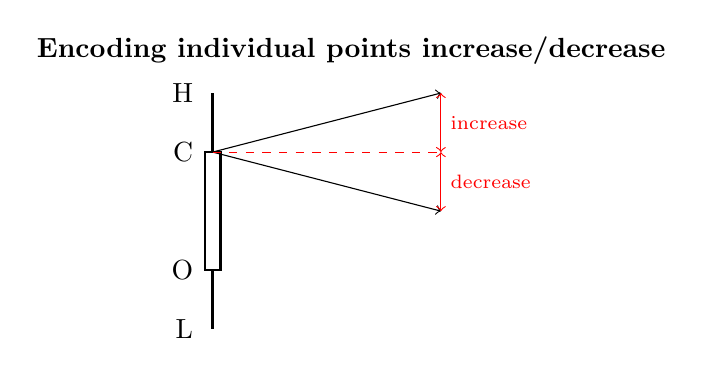
\begin{tikzpicture}
	\filldraw[thick, fill=white] (0, 0.75) rectangle (0.2, 2.25) ;
	\draw[thick] (0.1, 2.25) node[left] {C \hspace{3mm}} -- (0.1, 3) node[left] {H \hspace{3mm}};
	\draw[thick] (0.1, 0.75) node[left] {O \hspace{3mm}} -- (0.1, 0) node[left] {L \hspace{3mm}};
	\coordinate (C) at (0.1, 2.25);
	\coordinate (H) at (3, 3);
	\coordinate (L) at (3, 1.5);
	\draw [->] (C) -- (H);
	\draw [->] (C) -- (L);
	\draw[red, dashed] (C) -- (3, 2.25);
	\draw [red, <->] (3, 2.25) -- node[right] {\scriptsize increase} (H);
	\draw [red, <->] (3, 2.25) -- node[right] {\scriptsize decrease} (L);
	\node[above, font=\bfseries] at (current bounding box.north) {Encoding individual points increase/decrease};
	\end{tikzpicture}
\end{center}

To encode any change in direction (positive or negative) and its length we can consider seven possibilities: 0, 10, 25, 50, 75, 100 or  $>100$, for the new position or size.

To encode the change in position of a new candlestick we do need to consider the four points, and for each of them, the two different possibilities (increase or decrease --steady is coded as positive 0 change), and the grade of difference (one among the seven possible values). This encoding results therefore in $4 \times 2 \times 7 = 56$ possibilities.

\subsection{Range shift}

The other possibility is to encode the direction and size of the ranges $\overline{HL}$ and $\overline{OC}$ as shift in a given direction. The first couple of options are that the range will increase its values (both) or decrease them.

\begin{center}
	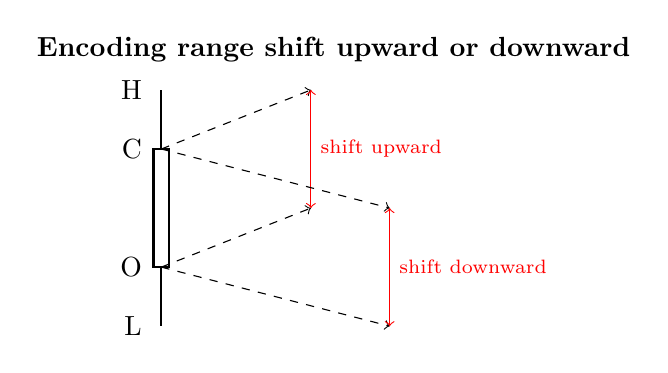
\begin{tikzpicture}
	\coordinate (C) at (0.1, 2.25);
	\coordinate (O) at (0.1, 0.75);
	\coordinate (H1) at (2, 3);
	\coordinate (L1) at (2, 1.5);
	\coordinate (H2) at (3, 1.5);
	\coordinate (L2) at (3, 0);
	
	\filldraw[thick, fill=white] (0, 0.75) rectangle (0.2, 2.25) ;
	\draw[thick] (0.1, 2.25) node[left] {C \hspace{3mm}} -- (0.1, 3) node[left] {H \hspace{3mm}};
	\draw[thick] (0.1, 0.75) node[left] {O \hspace{3mm}} -- (0.1, 0) node[left] {L \hspace{3mm}};
	
	\draw [dashed, ->] (C) -- (H1);
	\draw [dashed, ->] (O) -- (L1);
	\draw [red, <->] (L1) -- node[right] {\scriptsize shift upward} (H1);
	
	\draw [dashed, ->] (C) -- (H2);
	\draw [dashed, ->] (O) -- (L2);
	\draw [red, <->] (L2) -- node[right] {\scriptsize shift downward} (H2);
	
	\node[above, font=\bfseries] at (current bounding box.north) {Encoding range shift upward or downward};
	\end{tikzpicture}
\end{center}

But it can also increase or shrink its range without apparent shift upward or downward. In this case, the endpoints show a contradictory movement: one is increasing its value but the other one is decreasing it.

\begin{center}
	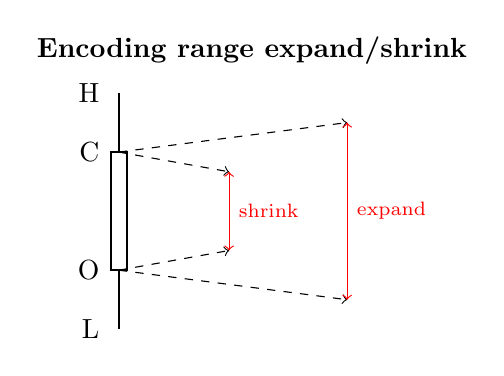
\begin{tikzpicture}
	\filldraw[thick, fill=white] (0, 0.75) rectangle (0.2, 2.25) ;
	\draw[thick] (0.1, 2.25) node[left] {C \hspace{3mm}} -- (0.1, 3) node[left] {H \hspace{3mm}};
	\draw[thick] (0.1, 0.75) node[left] {O \hspace{3mm}} -- (0.1, 0) node[left] {L \hspace{3mm}};
	\coordinate (C) at (0.1, 2.25);
	\coordinate (O) at (0.1, 0.75);
	\coordinate (H1) at (3, 2.625);
	\coordinate (L1) at (3, 0.375);
	\coordinate (H2) at (1.5, 2.0);
	\coordinate (L2) at (1.5, 1.0);
	
	\draw [dashed, ->] (C) -- (H1);
	\draw [dashed, ->] (O) -- (L1);
	\draw [red, <->] (L1) -- node[right] {\scriptsize expand} (H1);
	
	\draw [dashed, ->] (C) -- (H2);
	\draw [dashed, ->] (O) -- (L2);
	\draw [red, <->] (L2) -- node[right] {\scriptsize shrink} (H2);
	
	\node[above, font=\bfseries] at (current bounding box.north) {Encoding range expand/shrink};
	\end{tikzpicture}
\end{center}

All the possibilities enumerated in this section lead to nine different combinations:

\begin{itemize}
	\item shift upward, same size.
	\item shift upward, shrink.
	\item shift upward, expand.
	\item shift downward, same size.
	\item shift downward, shrink.
	\item shift downward, expand.
	\item shrink, no shift.
	\item expand, no shift.
	\item same size, no shift.
\end{itemize}

\subsection{Encoding movement}

To encode the 9 possibilities, a two letter encoding is proposed. The first one determines size behavior (shrink, expand or no change), and the second one the direction (upward, downward and no shift).

\begin{minted}[numbersep=5pt,gobble=2,frame=lines,framesep=2mm]{bash}
  {S|X|N}{U|D|N}
\end{minted}

\section{Optimal Encoding for maximum distance between distinct elements}

However, the total 45 possible candlestick codes need to be encoded in a way that maximizes the distance (hamming or levenhstein) between elements with big differences.

\begin{center}
	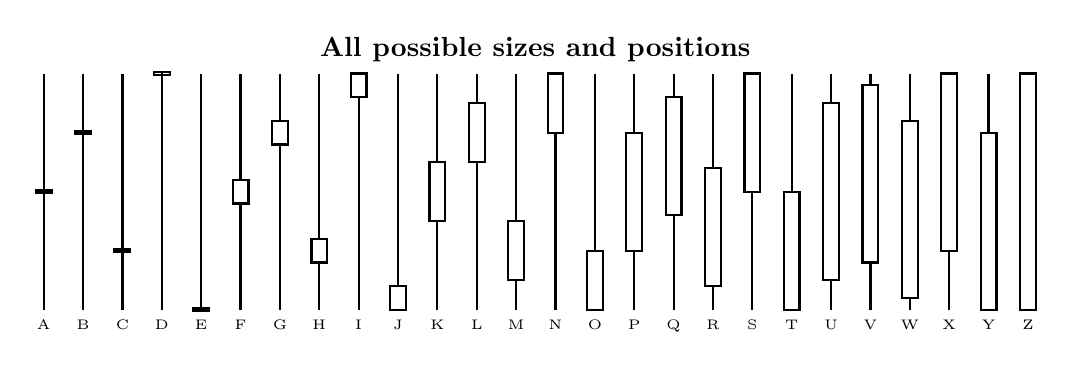
\begin{tikzpicture}

\filldraw[thick, fill=white] (0.000, 1.485) rectangle (0.200, 1.515);
\draw[thick] (0.100, 1.515) -- (0.100, 3);
\draw[thick] (0.100, 1.485) -- (0.100, 0) node[align=center, below] {\tiny A};
\filldraw[thick, fill=white] (0.500, 2.235) rectangle (0.700, 2.265);
\draw[thick] (0.600, 2.265) -- (0.600, 3);
\draw[thick] (0.600, 2.235) -- (0.600, 0) node[align=center, below] {\tiny B};
\filldraw[thick, fill=white] (1.000, 0.735) rectangle (1.200, 0.765);
\draw[thick] (1.100, 0.765) -- (1.100, 3);
\draw[thick] (1.100, 0.735) -- (1.100, 0) node[align=center, below] {\tiny C};
\filldraw[thick, fill=white] (1.500, 2.985) rectangle (1.700, 3.015);
\draw[thick] (1.600, 3.015) -- (1.600, 3);
\draw[thick] (1.600, 2.985) -- (1.600, 0) node[align=center, below] {\tiny D};
\filldraw[thick, fill=white] (2.000, -0.015) rectangle (2.200, 0.015);
\draw[thick] (2.100, 0.015) -- (2.100, 3);
\draw[thick] (2.100, -0.015) -- (2.100, 0) node[align=center, below] {\tiny E};
\filldraw[thick, fill=white] (2.500, 1.350) rectangle (2.700, 1.650);
\draw[thick] (2.600, 1.650) -- (2.600, 3);
\draw[thick] (2.600, 1.350) -- (2.600, 0) node[align=center, below] {\tiny F};
\filldraw[thick, fill=white] (3.000, 2.100) rectangle (3.200, 2.400);
\draw[thick] (3.100, 2.400) -- (3.100, 3);
\draw[thick] (3.100, 2.100) -- (3.100, 0) node[align=center, below] {\tiny G};
\filldraw[thick, fill=white] (3.500, 0.600) rectangle (3.700, 0.900);
\draw[thick] (3.600, 0.900) -- (3.600, 3);
\draw[thick] (3.600, 0.600) -- (3.600, 0) node[align=center, below] {\tiny H};
\filldraw[thick, fill=white] (4.000, 2.700) rectangle (4.200, 3.000);
\draw[thick] (4.100, 3.000) -- (4.100, 3);
\draw[thick] (4.100, 2.700) -- (4.100, 0) node[align=center, below] {\tiny I};
\filldraw[thick, fill=white] (4.500, 0.000) rectangle (4.700, 0.300);
\draw[thick] (4.600, 0.300) -- (4.600, 3);
\draw[thick] (4.600, 0.000) -- (4.600, 0) node[align=center, below] {\tiny J};
\filldraw[thick, fill=white] (5.000, 1.125) rectangle (5.200, 1.875);
\draw[thick] (5.100, 1.875) -- (5.100, 3);
\draw[thick] (5.100, 1.125) -- (5.100, 0) node[align=center, below] {\tiny K};
\filldraw[thick, fill=white] (5.500, 1.875) rectangle (5.700, 2.625);
\draw[thick] (5.600, 2.625) -- (5.600, 3);
\draw[thick] (5.600, 1.875) -- (5.600, 0) node[align=center, below] {\tiny L};
\filldraw[thick, fill=white] (6.000, 0.375) rectangle (6.200, 1.125);
\draw[thick] (6.100, 1.125) -- (6.100, 3);
\draw[thick] (6.100, 0.375) -- (6.100, 0) node[align=center, below] {\tiny M};
\filldraw[thick, fill=white] (6.500, 2.250) rectangle (6.700, 3.000);
\draw[thick] (6.600, 3.000) -- (6.600, 3);
\draw[thick] (6.600, 2.250) -- (6.600, 0) node[align=center, below] {\tiny N};
\filldraw[thick, fill=white] (7.000, 0.000) rectangle (7.200, 0.750);
\draw[thick] (7.100, 0.750) -- (7.100, 3);
\draw[thick] (7.100, 0.000) -- (7.100, 0) node[align=center, below] {\tiny O};
\filldraw[thick, fill=white] (7.500, 0.750) rectangle (7.700, 2.250);
\draw[thick] (7.600, 2.250) -- (7.600, 3);
\draw[thick] (7.600, 0.750) -- (7.600, 0) node[align=center, below] {\tiny P};
\filldraw[thick, fill=white] (8.000, 1.200) rectangle (8.200, 2.700);
\draw[thick] (8.100, 2.700) -- (8.100, 3);
\draw[thick] (8.100, 1.200) -- (8.100, 0) node[align=center, below] {\tiny Q};
\filldraw[thick, fill=white] (8.500, 0.300) rectangle (8.700, 1.800);
\draw[thick] (8.600, 1.800) -- (8.600, 3);
\draw[thick] (8.600, 0.300) -- (8.600, 0) node[align=center, below] {\tiny R};
\filldraw[thick, fill=white] (9.000, 1.500) rectangle (9.200, 3.000);
\draw[thick] (9.100, 3.000) -- (9.100, 3);
\draw[thick] (9.100, 1.500) -- (9.100, 0) node[align=center, below] {\tiny S};
\filldraw[thick, fill=white] (9.500, 0.000) rectangle (9.700, 1.500);
\draw[thick] (9.600, 1.500) -- (9.600, 3);
\draw[thick] (9.600, 0.000) -- (9.600, 0) node[align=center, below] {\tiny T};
\filldraw[thick, fill=white] (10.000, 0.375) rectangle (10.200, 2.625);
\draw[thick] (10.100, 2.625) -- (10.100, 3);
\draw[thick] (10.100, 0.375) -- (10.100, 0) node[align=center, below] {\tiny U};
\filldraw[thick, fill=white] (10.500, 0.600) rectangle (10.700, 2.850);
\draw[thick] (10.600, 2.850) -- (10.600, 3);
\draw[thick] (10.600, 0.600) -- (10.600, 0) node[align=center, below] {\tiny V};
\filldraw[thick, fill=white] (11.000, 0.150) rectangle (11.200, 2.400);
\draw[thick] (11.100, 2.400) -- (11.100, 3);
\draw[thick] (11.100, 0.150) -- (11.100, 0) node[align=center, below] {\tiny W};
\filldraw[thick, fill=white] (11.500, 0.750) rectangle (11.700, 3.000);
\draw[thick] (11.600, 3.000) -- (11.600, 3);
\draw[thick] (11.600, 0.750) -- (11.600, 0) node[align=center, below] {\tiny X};
\filldraw[thick, fill=white] (12.000, 0.000) rectangle (12.200, 2.250);
\draw[thick] (12.100, 2.250) -- (12.100, 3);
\draw[thick] (12.100, 0.000) -- (12.100, 0) node[align=center, below] {\tiny Y};
\filldraw[thick, fill=white] (12.500, 0.000) rectangle (12.700, 3.000);
\draw[thick] (12.600, 3.000) -- (12.600, 3);
\draw[thick] (12.600, 0.000) -- (12.600, 0) node[align=center, below] {\tiny Z};

		\node[above, font=\bfseries] at (current bounding box.north) {All possible sizes and positions};
	\end{tikzpicture}	
\end{center}

\end{document}
